\documentclass[a4paper, 10pt, ]{article}

\usepackage[slovak]{babel}

% ------------------------------

\usepackage[utf8]{inputenc}
\usepackage[T1]{fontenc}

\usepackage[left=4cm,
            right=4cm,
            top=2.1cm,
            bottom=2.6cm,
            footskip=7.5mm,
            twoside,
            marginparwidth=3.0cm,
            %showframe,
            ]{geometry}

\usepackage{graphicx}
\usepackage[dvipsnames]{xcolor}
% https://en.wikibooks.org/wiki/LaTeX/Colors

% ------------------------------

\usepackage{lmodern}

\usepackage[tt={oldstyle=false,proportional=true,monowidth}]{cfr-lm}
% https://mirror.szerverem.hu/ctan/fonts/cfr-lm/doc/cfr-lm.pdf

% ------------------------------

\usepackage{amsmath}
\usepackage{amssymb}
\usepackage{amsthm}

\usepackage{booktabs}
\usepackage{multirow}
\usepackage{array}
\usepackage{dcolumn}

\usepackage{natbib}

% ------------------------------

\hyphenpenalty=6000
\tolerance=1000

\def\naT{\mathsf{T}}

% ------------------------------

\makeatletter

    \def\@seccntformat#1{\protect\makebox[0pt][r]{\csname the#1\endcsname\hspace{4mm}}}

    \def\cleardoublepage{\clearpage\if@twoside \ifodd\c@page\else
    \hbox{}
    \vspace*{\fill}
    \begin{center}
    \phantom{}
    \end{center}
    \vspace{\fill}
    \thispagestyle{empty}
    \newpage
    \if@twocolumn\hbox{}\newpage\fi\fi\fi}

    \newcommand\figcaption{\def\@captype{figure}\caption}
    \newcommand\tabcaption{\def\@captype{table}\caption}

\makeatother

% ------------------------------

\usepackage{fancyhdr}
\fancypagestyle{plain}{%
\fancyhf{} % clear all header and footer fields
% \fancyfoot[C]{\sffamily {\bfseries \thepage}\ | {\scriptsize\oznacenieCasti}}
\fancyfoot[C]{\sffamily {\bfseries \thepage}{\color{Gray}\scriptsize$\,$z$\,$\pageref{LastPage}}\ | 
\includegraphics[height=5pt]{../../COMMONFILES/KUT_logo_v0.1.pdf}{\scriptsize\KUTporadoveCislo}}
\renewcommand{\headrulewidth}{0pt}
\renewcommand{\footrulewidth}{0pt}}
\pagestyle{plain}

% ------------------------------

\usepackage{titlesec}
\titleformat{\paragraph}[hang]{\sffamily  \bfseries}{}{0pt}{}
\titlespacing*{\paragraph}{0mm}{3mm}{1mm}
\titlespacing*{\subparagraph}{0mm}{3mm}{1mm}

\titleformat*{\section}{\sffamily\Large\bfseries}
\titleformat*{\subsection}{\sffamily\large\bfseries}
\titleformat*{\subsubsection}{\sffamily\normalsize\bfseries}


% ------------------------------

\PassOptionsToPackage{hyphens}{url}
\usepackage[pdfauthor={},
            pdftitle={},
            pdfsubject={},
            pdfkeywords={},
            % hidelinks,
            colorlinks=false,
            breaklinks,
            ]{hyperref}


% ------------------------------

\graphicspath{%
{../fig_standalone/}%
{../../PY/fig/}%
{../../ML/fig/}%
{./fig/}%
}

% ------------------------------

\usepackage{enumitem}

\usepackage{lettrine}

% ------------------------------

\usepackage{lastpage}

\usepackage{microtype}

% ------------------------------

\usepackage{algorithm}
\usepackage[noend]{algpseudocode}
\makeatletter
\renewcommand{\ALG@name}{Algoritmus}
\makeatother
\usepackage{amsmath}
\usepackage{bbold}
\usepackage{calc}
\usepackage{dsfont}
\usepackage{mathtools}
\usepackage{tabto}


\newcommand{\mr}[1]{\mathrm{#1}}
\newcommand{\bs}[1]{\boldsymbol{#1}}
\newcommand{\bm}[1]{\mathbf{#1}}

\newcommand{\diff}[2]{\frac{\Delta #1}{\Delta #2}}
\newcommand{\der}[2]{\frac{d #1}{d #2}}
\newcommand{\parder}[2]{\frac{\partial #1}{\partial #2}}

\newcommand{\argmax}[0]{\mr{argmax}}
\newcommand{\diag}[0]{\mr{diag}}
\newcommand{\rank}[0]{\mr{rank}}
\newcommand{\trace}[0]{\mr{tr}}

\renewcommand{\Re}{\mr{Re}}
\renewcommand{\Im}{\mr{Im}}


\theoremstyle{definition}
\newtheorem{definition}{Definícia}[section]
\newtheorem{theorem}{Veta}[section]
\newtheorem{lemma}[theorem]{Lemma}
\newtheorem{example}{Príklad}[section]
\renewcommand*{\proofname}{Dôkaz}

% ------------------------------

\usepackage{siunitx}

% -----------------------------------------------------------------------------

\def\oznacenieCelku{Kolekcia učebných textov}

% -----------------------------------------------------------------------------


\def\KUTporadoveCislo{devAS0}

\def\oznacenieVerzie{v1.0}
% \def\oznacenieVerzie{\phantom{v1.0}}

\def\mesiacRok{august 2025}

\def\authorslabel{RJ}






% -----------------------------------------------------------------------------

\begin{document}

% -----------------------------------------------------------------------------
% Uvodny nadpis

\noindent
\parbox[t][18mm][c]{0.3\textwidth}{%
    \raisebox{-0.9\height}{%
        \phantom{.}
\includegraphics[height=18mm]{./COMMONFILES/URKFEIlogo.pdf}%
    }%
}%
\parbox[t][18mm][c]{0.7\textwidth}{%
    \raggedleft

    \sffamily
    \fontsize{16pt}{18pt}
    \fontseries{sbc}
    \selectfont

    \noindent
    \textcolor[rgb]{0.75, 0.75, 0.75}{\textls[25]{\oznacenieCelku}}
}%

\noindent
\parbox[t][16mm][b]{0.5\textwidth}{%
    \raggedright

    \color{Gray}
    \sffamily

    \fontsize{12pt}{12pt}
    \selectfont
    \mesiacRok

    \fontsize{6pt}{10pt}
    \selectfont
    \href{https://github.com/OkoliePracovnehoBodu/KUT}{github.com/OkoliePracovnehoBodu/KUT}

    \fontsize{8pt}{10pt}
    \selectfont
    \authorslabel




}%
\parbox[t][16mm][b]{0.5\textwidth}{%
    \raggedleft

    \sffamily

    \fontsize{6pt}{6pt}
    \selectfont

    \textcolor[rgb]{0.68, 0.68, 0.68}{\oznacenieVerzie}


    \fontsize{14pt}{14pt}
    \selectfont

    \bfseries

    
\includegraphics[height=12pt]{./COMMONFILES/KUT_logo_v0.1.pdf}%
    {%
        \textls[-50]{\KUTporadoveCislo}
    }%
}%

% -----------------------------------------------------------------------------




\vspace{6mm}

% ---------------------------------------------
\sffamily
\bfseries
\fontsize{18pt}{21pt}
\selectfont

\begin{flushleft}
    Laboratórne zariadenie AeroShield:\\ orientačný prehľad
\end{flushleft}

\bigskip

% -----------------------------------------------------------------------------
\normalsize
\normalfont
% -----------------------------------------------------------------------------

\lstset{style=mystyle}










\noindent
\lettrine[lines=1, nindent=1pt, loversize=0.0]{C}{ieľom}
textu je opis laboratórneho zariadenia AeroShield predstavujúceho fyzický model spojitého dynamického systému.


\section{Opis dynamického systému}

AeroShield (daľej len \emph{AS}) je laboratórne zariadenie predstavujúce reálny dynamický systém. Pozostáva z jednoramenného kývadla, malého jednosmerného motora s rotorom na vystupnom hriadeli - uloženého na nevotknutom konci kývajúceho sa ramena. Následne je výstup snímaní magnetickým rotačným enkóderom AS5600, ktorý zabezpečuje presné meranie uhlovej polohy ramena a osadeného potenciometru, ktorý možno použiť na riadenie referenčnej veličiny systému alebo manuálne riadenie motora - záleži od implementácie, rovnako sa signál z potenciometra dá použiť na predčasné ukončenie merania.

Systém má jeden vstupný signál a jeden výstupný signál. Výstupný signál je priamo úmerný uhlovej polohe ramena, ktorá je snímaná enkóderom. Vstupný signál ovláda napájanie motora.

Polohou potenciometra je v podstate signál, ktorý vie uživateľ použiť na rôzne účeli, ale nijak ne ovplyvňuje systém ako taký, bez toho aby si to uživateľ sám neimplementoval.



\section{Rozsahy a jednotky signálov}

Z opisu predmetného dynamického systému vyplýva, že systém má jeden výstupný signál, jeden vstupný signál a manuálne nastaviteľnú prevádzkovú podmienku.

Vstupný a výstupný signál nadobúdajú hodnoty v~rozsahu $0$ až $10$ pričom ide o~napäťové signály vo voltoch [V].

Prevádzkové podmienka systému sa nastavuje manuálne otáčaním potenciometra. Signál o polohe potenciometra nadobúda hodnoty v rozsahu $0$ [V] až $10$ [V].





\begin{center}

    \vspace{-10pt}

    \tabcaption{Rozsahy a jednotky signálov}
    \label{tab:rozsahy_a_jednotky_signalu}

    \lstyle

    \begin{tabular*}{\textwidth}{@{ \extracolsep{\fill}} lll}
        \toprule
        Signál & Rozsah hodnôt & Jednotka \\
        \midrule
        Vstup & $0$ až $10$ & V (volt) \\
        Výstup & $0$ až $10$ & V (volt) \\
        Prevádzkové nastavenie & $0$ až $10$ & V (volt) \\
        \bottomrule
    \end{tabular*}


\end{center}







\section{Schematické znázornenie systému}


\begin{center}

    \vbox{%


        \makebox[\textwidth][c]{%
            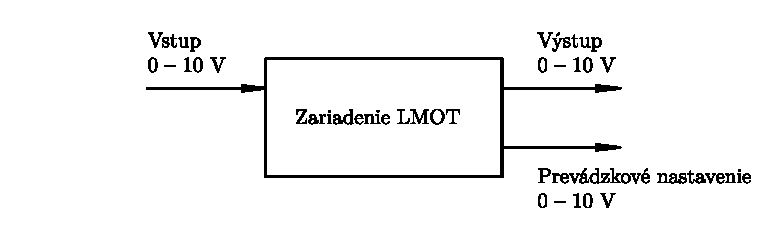
\includegraphics{LMOT_sch1.pdf}
        }

        \figcaption{
            Signály systému LMOT.
        }
        \label{LMOT_sch1}
    }%vbox

\end{center}


\begin{center}

    \vbox{%


        \makebox[\textwidth][c]{%
            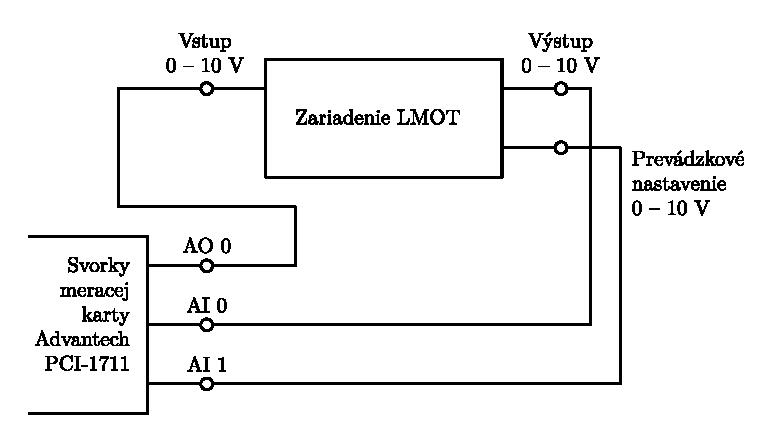
\includegraphics{LMOT_sch2.pdf}
        }

        \figcaption{
            Schéma pripojenia laboratórneho zariadenia k svorkám meracej karty Advantech PCI-1711, pričom AO~$0$ je analógový výstup meracej karty a~AI~$0$, AI~$1$ sú analógové vstupy meracej karty.
        }
        \label{LMOT_sch2}
    }%vbox

\end{center}



\section{Fotografie}

Zoznam fotografií:

\begin{itemize}
    \item Obr. \ref{IMG_6874_toPDF}: Celkový pohľad na laboratórne zariadenie LMOT.
    \item Obr. \ref{IMG_6922_toPDF}: Motor a tachodynamo.
    \item Obr. \ref{IMG_6941_toPDF}: Elektronické obvody zariadenia.
    \item Obr. \ref{IMG_6931_toPDF}: Predný panel so svorkami a potenciometrom.
\end{itemize}





\noindent
\vbox{%

    \makebox[\textwidth][c]{%
        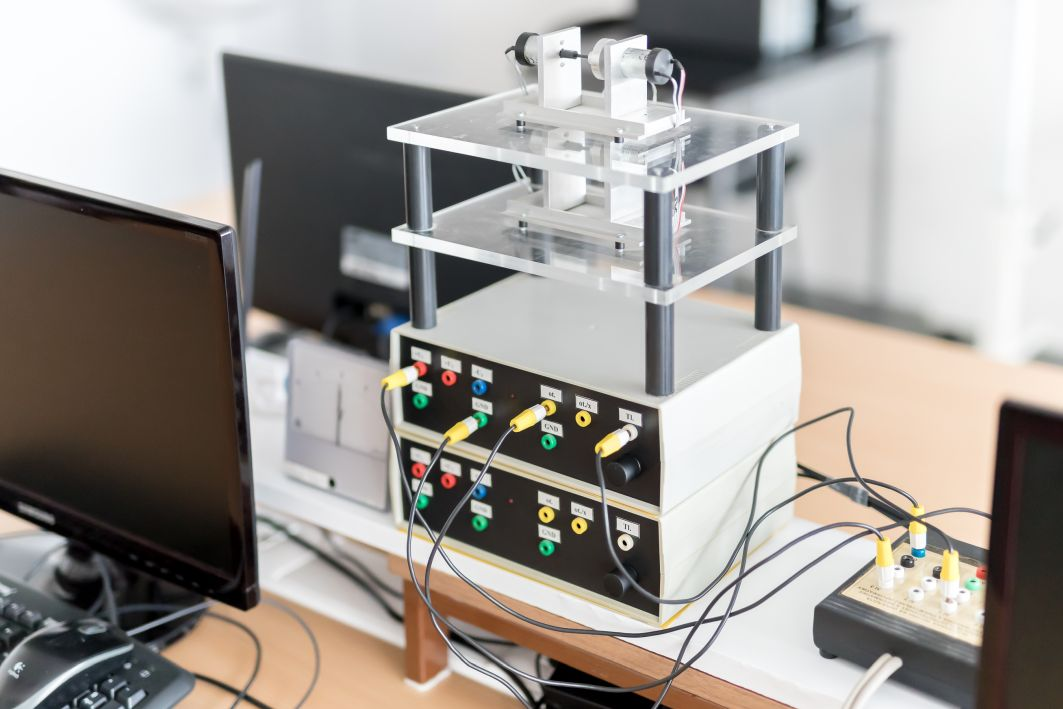
\includegraphics{IMG_6874_toPDF.jpg}
    }

    \figcaption{
        Celkový pohľad na laboratórne zariadenie LMOT.
    }

    \vspace{12pt}

    \label{IMG_6874_toPDF}
}%vbox



\noindent
\vbox{%

    \makebox[\textwidth][c]{%
        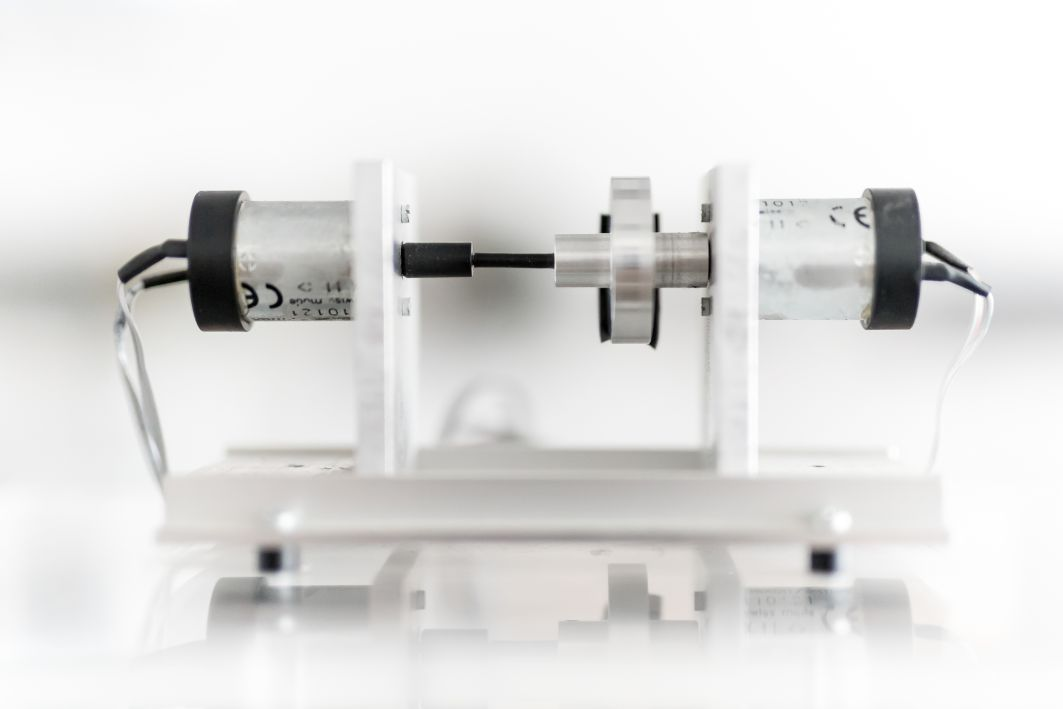
\includegraphics{IMG_6922_toPDF.jpg}
    }

    \figcaption{
        Motor a tachodynamo.
    }

    \vspace{12pt}

    \label{IMG_6922_toPDF}
}%vbox




\noindent
\vbox{%

    \makebox[\textwidth][c]{%
        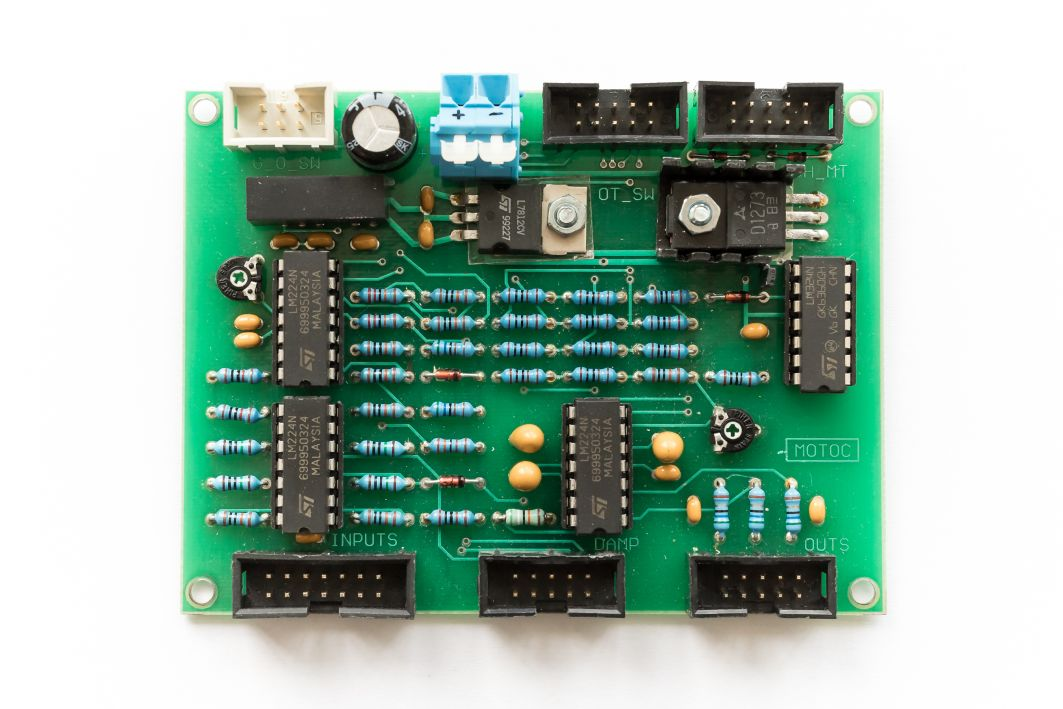
\includegraphics{IMG_6941_toPDF.jpg}
    }

    \figcaption{
        Elektronické obvody zariadenia.
    }

    \vspace{12pt}

    \label{IMG_6941_toPDF}
}%vbox




\noindent
\vbox{%

    \makebox[\textwidth][c]{%
        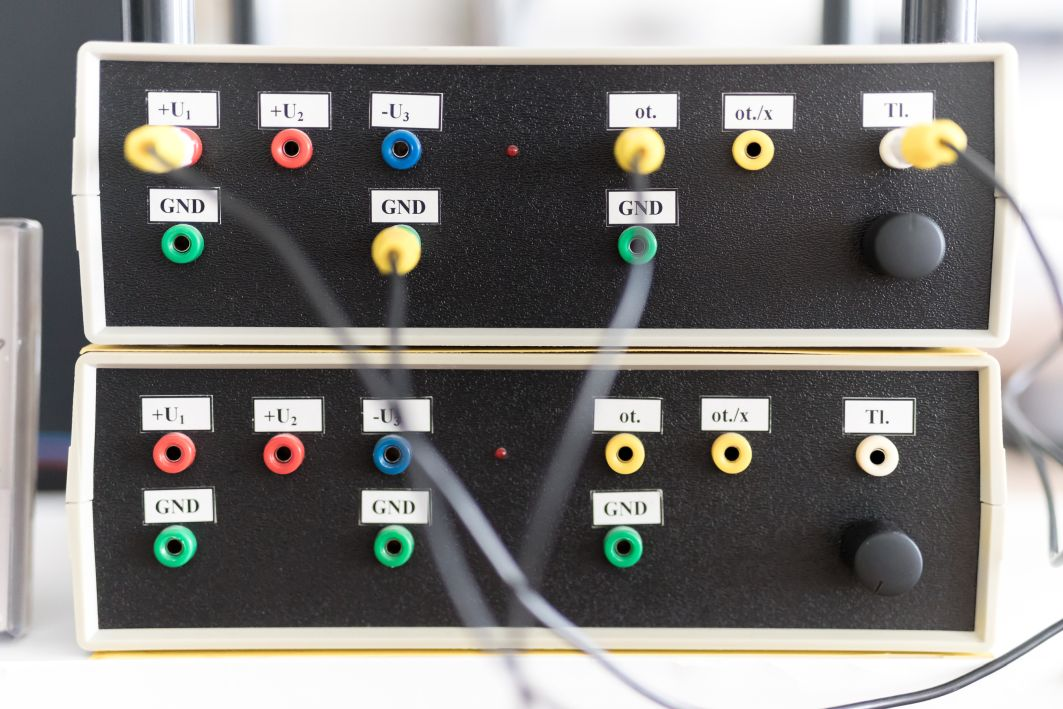
\includegraphics{IMG_6931_toPDF.jpg}
    }

    \figcaption{
        Predný panel so svorkami a potenciometrom.
    }

    \vspace{12pt}

    \label{IMG_6931_toPDF}
}%vbox

























































% -----------------------------------------------------------------------------

\end{document}

% -----------------------------------------------------------------------------